\documentclass[9pt,a4paper]{jsarticle} 

\usepackage[left=15mm,right=15mm,top=15mm,bottom=20mm]{geometry}
\pagestyle{empty} 

\usepackage{amsmath} 
\usepackage{amssymb}
\usepackage{ascmac} 
\usepackage{epsfig}
\usepackage{listings,jlisting}

\title{{\bf Information Visualization W15: Final Tasks}}
\author{{\bf
	\begin{tabular}{c}
	167X009X $B:e8}(B $B:K(B\\
	\end{tabular}
}}
\date{2016$BG/(B6$B7n(B17$BF|Ds=PJ,(B} 

\begin{document} 
\maketitle

\section*{$B%W%m%0%i%`35MW(B}
$B%V%i%&%6>e$G(BBoxGeometry$B$N%W%m%Q%F%#CM$rF0E*$KJQ99$G$-$k%W%m%0%i%`$r:n@.$7$?!%%Q%i%a!<%?$rJQ2=$5$;$k$?$a!$<x6H$G$b>R2p$N$"$C$?(Bdat.GUI$B$rF3F~$7$F$$$k!%(B
\section*{$B%=!<%9%3!<%I(B}
$B:#2s;HMQ$7$?%=!<%9%3!<%I$r7G:\$9$k!%;HMQ$7$F$$$k%i%$%V%i%j$O:Y$+$J:n6H$N$?$a$N(BjQuery$B$H!$(BThreeJS$B$+$i$O(Bthree.min.js$B!$(BDetector.js$B!$(BOrbitControls.js$B!$(Bdat.gui.min.js$B$rFI$_9~$s$G$$$k!%4J0WE*$J2r@b$N$?$a!$3F%;%s%F%s%9$K35MW%3%a%s%H$rCm<a$7$F$*$/!%(B

\begin{lstlisting}[basicstyle=\ttfamily\footnotesize, frame=single]
(function($){
	var width = 640;  
	var height = 480; 
	var scene,camera,renderer,controls,geoObj,mesh;
	 
	function main(){
		//WebGL$B4D6-3NG'(B
		if(!Detector.webgl)Detector.addGetWebGLMessage();
		//GUI$BF3F~(B
		var gui = new dat.GUI();

		scene = new THREE.Scene();
 
		// $B%+%a%i(B:$BF);kEj1F(B
		camera = new THREE.PerspectiveCamera( 60, width/height, 0.001, 2000);
		scene.add(camera);
		camera.position.set( 0, 20, 40);
 
		// $B%l%s%@%i!<(B
		renderer = new THREE.WebGLRenderer({antialias: true});
		renderer.setSize(width,height);
		renderer.setPixelRatio( window.devicePixelRatio);
		renderer.shadowMap.enabled = true;
		document.body.appendChild( renderer.domElement );
 
		// $B%8%*%a%H%j!<(B
		var material = new THREE.MeshLambertMaterial({color: 0xFFA500});
		mesh = new THREE.Mesh();
		mesh.material = material;
		mesh.position.set(0,0,0);
		mesh.castShadow = true;
		scene.add(mesh);
		
		// $B%Q%i%a!<%?!<@_CV(B
		geoObj = new geoCtrl();
		var folder = gui.addFolder('BoxGeometry')
		folder.add( geoObj, 'x', 10, 80 ).onChange( setGeoVal);
		folder.add( geoObj, 'y', 10, 80 ).onChange( setGeoVal);
		folder.add( geoObj, 'z', 10, 80 ).onChange( setGeoVal);
		setGeoVal();
		
		// $B<+A38w(B
		var ambientLight = new THREE.AmbientLight( 0xDDDDCC, 0.8);

		// $B%9%]%C%H%i%$%H(B
		var spotLight = new THREE.SpotLight(0xFFFFFF,1.2,0);
		spotLight.castShadow = true;
		spotLight.position.set( 10, 30, 30);
		scene.add(ambientLight,spotLight);
 
		//$B%3%s%H%m!<%i!<(B
		controls = new THREE.OrbitControls(camera);
		controls.maxDistance = 100;
		controls.maxPolarAngle = Math.PI * 0.48;
		
		resizeSet();
		setTimeout(resize, 1);

		//$B<+F02sE>(B
		controls.autoRotate = true;
		controls.autoRotateSpeed = 2.0;
 
		rendering();
	}
 
	//GUI$B%Q%i%a!<%?$N=i4|CM(B
	var geoCtrl = function(){
		this.x = 20;
		this.y = 20;
		this.z = 20;
	};
	
	//GUI$B%Q%i%a!<%?$N=`Hw(B
	function setGeoVal(){
		mesh.geometry.dispose();
		mesh.geometry = new THREE.BoxGeometry( geoObj.x, geoObj.y ,geoObj.z );
	}
 
	function rendering(){
		requestAnimationFrame(rendering);
		controls.update();
		renderer.render( scene, camera);
	}
 
	function resizeSet(){
		var queue = null; // $B%-%e!<$r%9%H%C%/(B 
    	var wait = 300; // 0.3$BIC8e$K<B9T(B 
    	window.addEventListener( 'resize', function() {
    		clearTimeout( queue );
    		queue = setTimeout(function() {
    				resize();
    		}, wait );
    	}, false );
    };
	function resize(){
		var width = window.innerWidth;
		var height = window.innerHeight;
		camera.aspect = width/height;
		camera.updateProjectionMatrix();
		renderer.setSize(width, height);
	}
 
	$(function(){
		main();
	});
})(jQuery);
\end{lstlisting}

\subsection*{$B<B9T7k2L(B}

$B%W%m%0%i%`$r<B9T$5$;$k$H!"?^(B\ref{1}$B$N$h$&$J2hLL$,I=<($5$l$k!#3+;OD>8e$N(BBoxGeometry$B$N7A>u$O(B$(x:y:z)=(20\times20\times20)$$B$NN)J}BN$G$"$k!#(B

\begin{figure}[htbp]
  \begin{center} %$B%;%s%?%j%s%0$9$k(B
    \includegraphics[clip,width=10.0cm]{2.eps}
    \caption{$B%W%m%0%i%`<B9TD>8e$N(BBoxGeometry} %$B%?%$%H%k$r$D$1$k(B
    \label{1} %$B%i%Y%k$r$D$1?^$N;2>H$r2DG=$K$9$k(B
  \end{center}
\end{figure}

$B2hLL1&>e$N%\%C%/%9$N%7!<%/%P!<$rA08e$5$;$k$H!"3F<4J}8~$NJU$NBg$-$5$r(B$10\leqq\cdot\leqq80$$B$NHO0O$GJQ99$5$;$k$3$H$,$G$-$k!#$J$*!"?^(B\ref{2}$B$O!"(B$y=35$$B$KJQ99$7$?Nc$G$"$k!#(B

\begin{figure}[htbp]
  \begin{center} %$B%;%s%?%j%s%0$9$k(B
    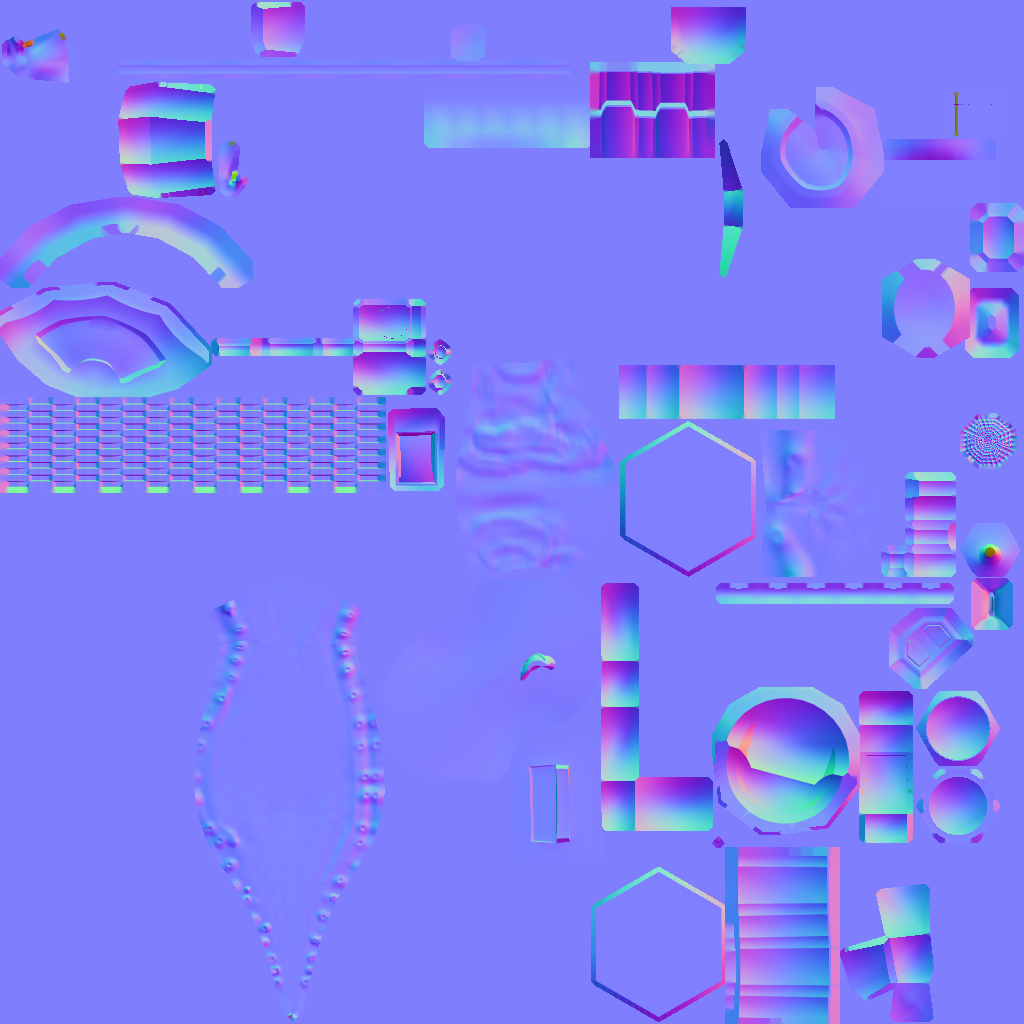
\includegraphics[clip,width=10.0cm]{1.eps}
    \caption{GUI$B$G%Q%i%a!<%?$rJQ2=$5$;$?(BBoxGeometry} %$B%?%$%H%k$r$D$1$k(B
    \label{2} %$B%i%Y%k$r$D$1?^$N;2>H$r2DG=$K$9$k(B
  \end{center}
\end{figure}

\end{document}
